% Numeración del capítulo: 5.
\setcounter{chapter}{4}

\chapter{Aplicación web para la gestión documental}\label{chap:web}

Este capítulo describe el cuarto componente del sistema: la aplicación web que integra el \textit{pipeline} de preprocesamiento del capítulo~\ref{chap:preprocesamiento} y el modelo de reconocimiento del capítulo~\ref{chap:modelo} en una herramienta accesible para los usuarios finales del centro Juan Marinello. La aplicación ofrece un flujo completo que comprende la subida de facsímiles, el procesamiento OCR automático, la revisión manual de las transcripciones que el modelo produce, y la exportación de los resultados a formatos estándar. El capítulo cuenta con siete secciones. La sección~\ref{sec:arq-web} presenta la arquitectura general y la pila tecnológica que la sustenta. La sección~\ref{sec:modelo-datos} describe el modelo de datos relacional y el formato XML~\cite{w3c2008xml} que alberga las transcripciones. La sección~\ref{sec:roles-acceso} detalla el sistema de roles y control de acceso. La sección~\ref{sec:flujo-digitalizacion} expone el flujo completo de digitalización desde la subida hasta la exportación. La sección~\ref{sec:integracion-ocr} describe la integración del modelo de reconocimiento. La sección~\ref{sec:editor} presenta el editor de revisión de transcripciones. La sección~\ref{sec:formato-xml} desarrolla el formato XML que el sistema emplea para almacenar las transcripciones de las páginas.

% -----------------------------------------------------------------------------
\section{Arquitectura general y pila tecnológica}
\label{sec:arq-web}

El trabajo construyó la aplicación sobre Django, el \textit{framework} web en Python que la sección~\ref{subsec:django-mvt} del capítulo~\ref{chap:estado-arte} introdujo. La madurez del \textit{framework}, la productividad que ofrece el patrón Modelo-Vista-Plantilla~\cite{django2024mvt}, y la disponibilidad de bibliotecas auxiliares para autenticación, validación de formularios y administración de bases de datos justifican la elección. La tabla~\ref{tab:pila-tecnologica} resume la pila completa que sustenta el sistema.

\begin{table}[!htbp]
	\centering
	\caption{Pila tecnológica de la aplicación web.}
	\label{tab:pila-tecnologica}
	\begin{tabular}{ll}
		\toprule
		\textbf{Capa} & \textbf{Tecnología} \\
		\midrule
		\textit{Framework} web        & Django 4.2 \\
		Lenguaje de programación      & Python 3.10 o superior \\
		Base de datos relacional      & PostgreSQL 13 o superior \\
		Persistencia de transcripciones & XML por página en sistema de ficheros \\
		Persistencia de facsímiles    & Imágenes en sistema de ficheros \\
		Procesamiento OCR             & PyTorch sobre el modelo del capítulo~\ref{chap:modelo} \\
		\textit{Pipeline} de imagen   & OpenCV y NumPy, según capítulo~\ref{chap:preprocesamiento} \\
		Procesado en \textit{background} & Hilos de Python con la API \textit{threading} \\
		\bottomrule
	\end{tabular}
\end{table}

El proyecto se organiza en cinco aplicaciones que la terminología de Django llama \textit{apps}. La aplicación \textit{accounts} gestiona los usuarios y la autenticación. La aplicación \textit{documents} gestiona los documentos, las páginas y las transcripciones. La aplicación \textit{ocr} encapsula el motor de reconocimiento y las tareas en \textit{background} que lo invocan. La aplicación \textit{stats} acumula las métricas de uso. La aplicación \textit{search} implementa la búsqueda de documentos por contenido, módulo que queda fuera del alcance del trabajo y que el resto del capítulo no aborda. La figura~\ref{fig:apps-diagrama} muestra las cinco aplicaciones y las dependencias entre ellas.

\begin{figure}[!htbp]
	\centering
	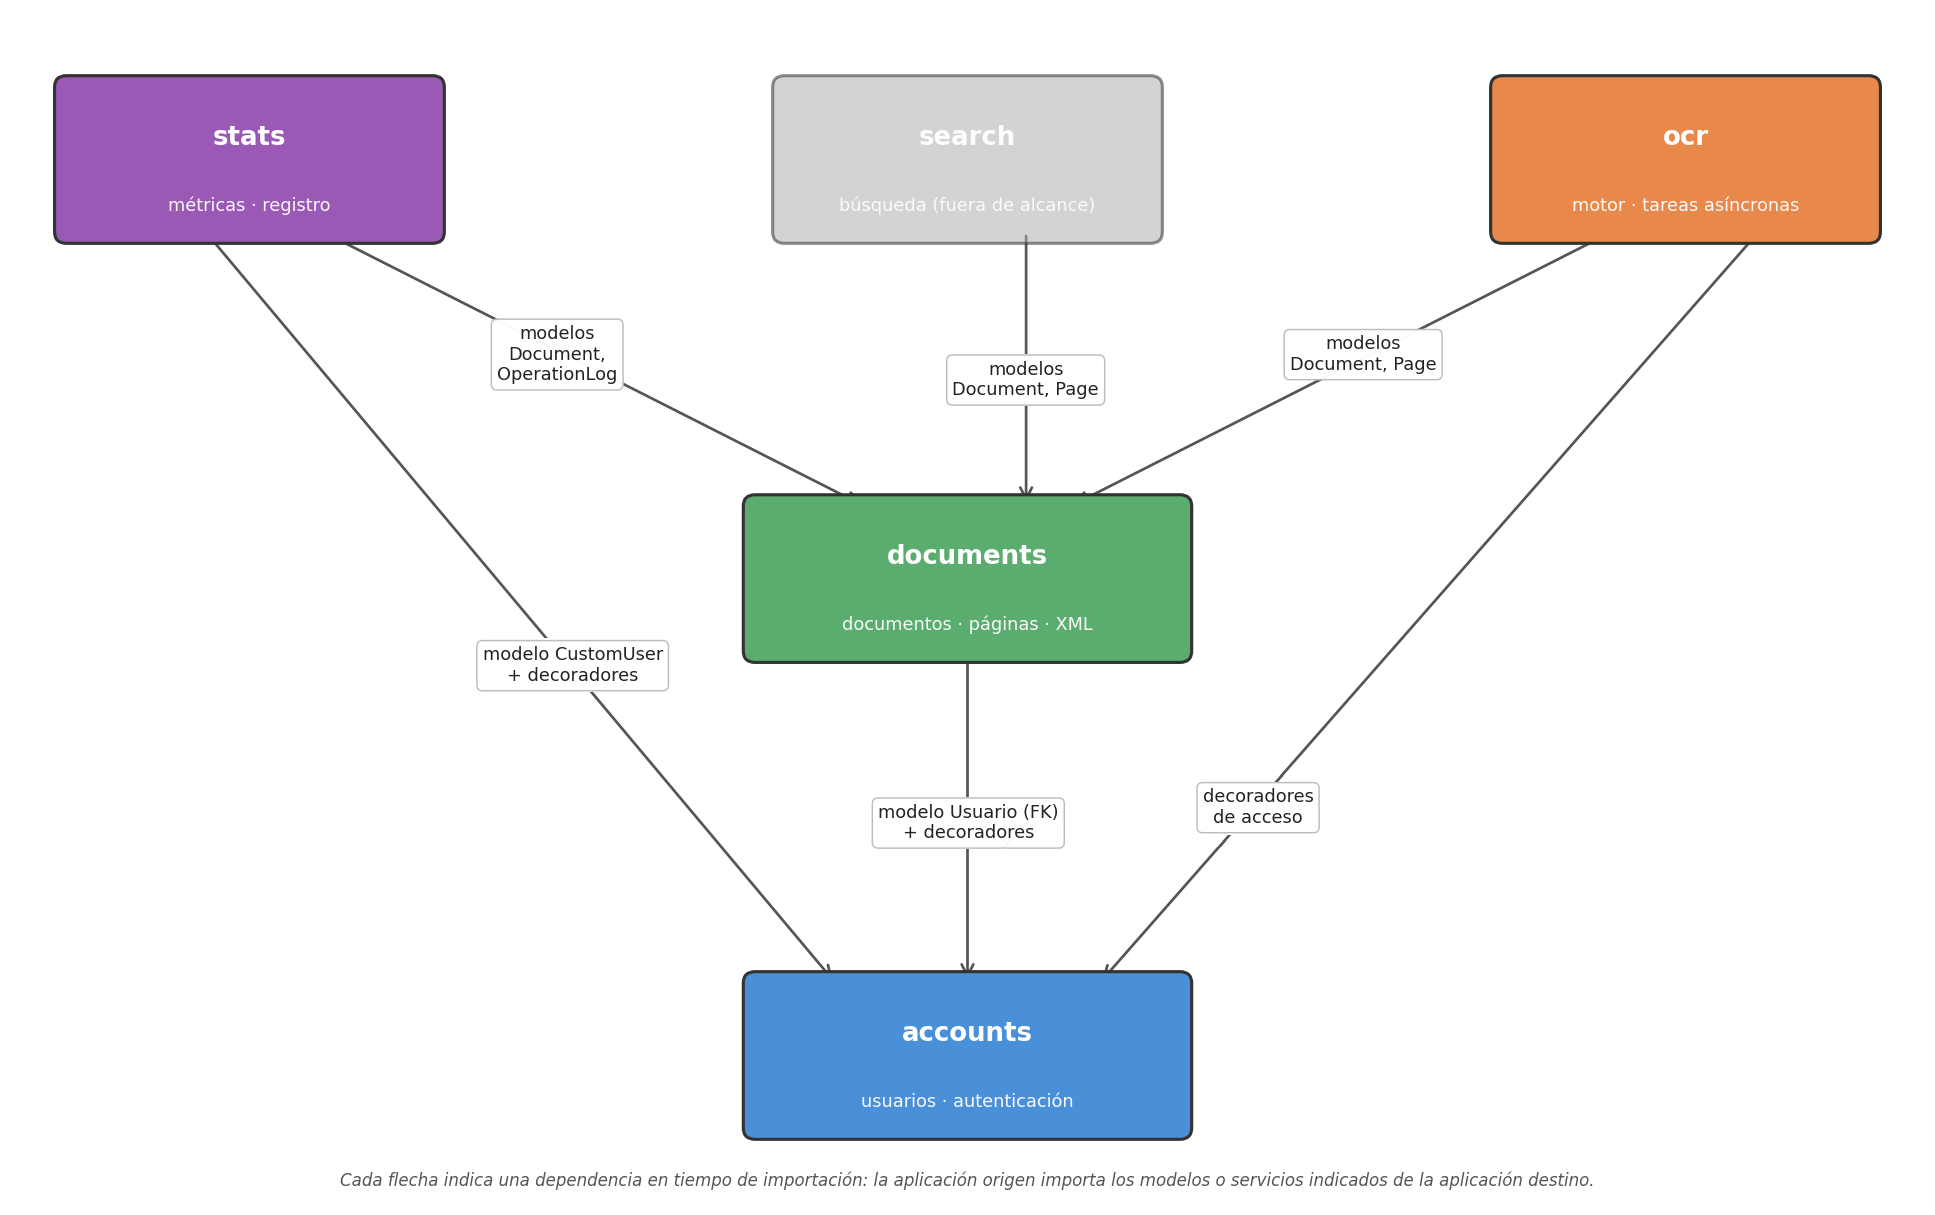
\includegraphics[width=0.88\textwidth]{Graphics/apps_diagram.png}
	\caption{Diagrama de dependencias entre las cinco aplicaciones del proyecto Django. Cada flecha apunta de la aplicación que importa hacia la que provee, y la etiqueta identifica los modelos o servicios concretos que se importan. La aplicación \textit{search} se incluye por completitud pero queda fuera del alcance de esta tesis.}
	\label{fig:apps-diagrama}
\end{figure}

La separación en cinco aplicaciones responde a tres objetivos. El primero es el aislamiento de responsabilidades: cada aplicación encapsula un dominio funcional con sus modelos de datos, vistas y las plantillas que les corresponden, sin acoplamiento innecesario al resto. El segundo objetivo es la facilidad de mantenimiento: cuando una funcionalidad requiere modificación, el desarrollador puede localizar el código sin recorrer el proyecto completo. El tercer objetivo es la reusabilidad: una aplicación bien aislada podría incorporarse a otro proyecto Django con cambios mínimos.

La persistencia adopta una estrategia híbrida. PostgreSQL almacena los datos relacionales que requieren consultas eficientes, transacciones e integridad referencial: usuarios, metadatos de documentos, metadatos de páginas (la ruta al facsímil, el número de orden dentro del documento y el estado del procesamiento OCR), registros de operaciones y métricas de uso. El sistema de ficheros almacena los datos voluminosos que el sistema consulta mayoritariamente por su identificador y rara vez por sus contenidos: imágenes facsimilares y transcripciones en formato XML. La estrategia evita sobrecargar la base de datos con \textit{blobs} binarios y mantiene la facilidad de inspección manual que requiere el flujo de digitalización de documentos.

% -----------------------------------------------------------------------------
\section{Modelo de datos}
\label{sec:modelo-datos}

El modelo de datos relacional comprende cuatro entidades principales que enlazan mediante claves foráneas: el usuario, el documento, la página y el registro de operaciones. La figura~\ref{fig:mer-diagrama} resume el Modelo Entidad-Relación, con los atributos de cada entidad y las relaciones de cardinalidad que las conectan. El esquema completo de la base de datos lo gestiona el sistema de migraciones de Django, que mantiene la coherencia entre los modelos del código fuente y las tablas físicas.

El esquema satisface las condiciones de la forma normal de Boyce-Codd~\cite{codd1972normalization}. La primera forma normal queda satisfecha por construcción: todos los atributos toman valores atómicos, sin estructuras anidadas ni listas dentro de campos individuales. La segunda forma normal queda satisfecha trivialmente porque las claves primarias de las cuatro entidades son simples (el campo \texttt{id} en todos los casos), por lo que no existen dependencias parciales sobre claves compuestas. La tercera forma normal queda satisfecha por inspección directa: ningún atributo no clave de una entidad depende transitivamente de la clave primaria a través de otro atributo no clave. Los atributos \texttt{created\_by\_id} y \texttt{last\_modified\_by\_id} de la entidad documento, por ejemplo, son claves foráneas a la entidad usuario y no derivan ningún otro atributo de la propia entidad documento. La forma normal de Boyce-Codd queda satisfecha porque cada dependencia funcional del esquema tiene como determinante una superclave: la clave primaria \texttt{id} en todas las entidades, o la pareja \texttt{(document\_id, order)} en la entidad página, que el esquema declara como restricción única y que constituye una clave candidata alternativa.

Dos decisiones de diseño del esquema merecen justificación explícita. La primera es la representación del rol del usuario como un atributo de tipo enumerado con tres valores fijos (\textit{trabajador}, \textit{administrador} y \textit{administrador principal}), en lugar de una entidad \textit{Rol} separada con su propia tabla y referencias mediante clave foránea. La elección responde a que los tres roles son categorías institucionales cerradas, sin atributos propios que justifiquen una entidad aparte: el rol carece de descripción extendida, de almacenar datos o metadatos de permisos explícitos que el sistema requiera vincular al rol y que pudieran crecer con el tiempo. La lógica de cada rol vive en el código, no en la base de datos, y se materializa en los decoradores de control de acceso que la sección~\ref{sec:roles-acceso} describe. La decisión simplifica el esquema y elimina una unión adicional en cada consulta sobre usuarios, a cambio de exigir una migración del código y de la base de datos si en el futuro el centro necesita añadir o eliminar roles. La consecuencia es aceptable dado el carácter estable de la estructura institucional del archivo.

La segunda decisión es la ausencia de campos que almacenen las rutas a los ficheros XML de transcripción y a las visualizaciones de segmentación de líneas. La razón es que el identificador del documento y el número de orden de la página determinan unívocamente la ruta de cualquiera de los ficheros. La función \texttt{transcript\_path(document\_id, page\_order)} del módulo de transcripciones construye la ruta de la forma
\begin{quote}
	\centering
	\texttt{\{MEDIA\_ROOT\}/transcripts/\{document\_id\}/page\_\{order:03d\}.xml}
\end{quote}
y una función análoga construye la ruta para visualizar la segmentación que el sistema guarda en caché bajo el subdirectorio \texttt{segmentation/}. La ruta, por tanto, deriva de otros atributos de la página, y almacenarla como campo violaría la tercera forma normal al introducir una dependencia transitiva entre atributos no clave. La aproximación garantiza que cada página tenga su transcripción y su visualización en una ubicación canónica y predecible, sin posibilidad de inconsistencia entre la base de datos y el sistema de ficheros.

\begin{figure}[!htbp]
	\centering
	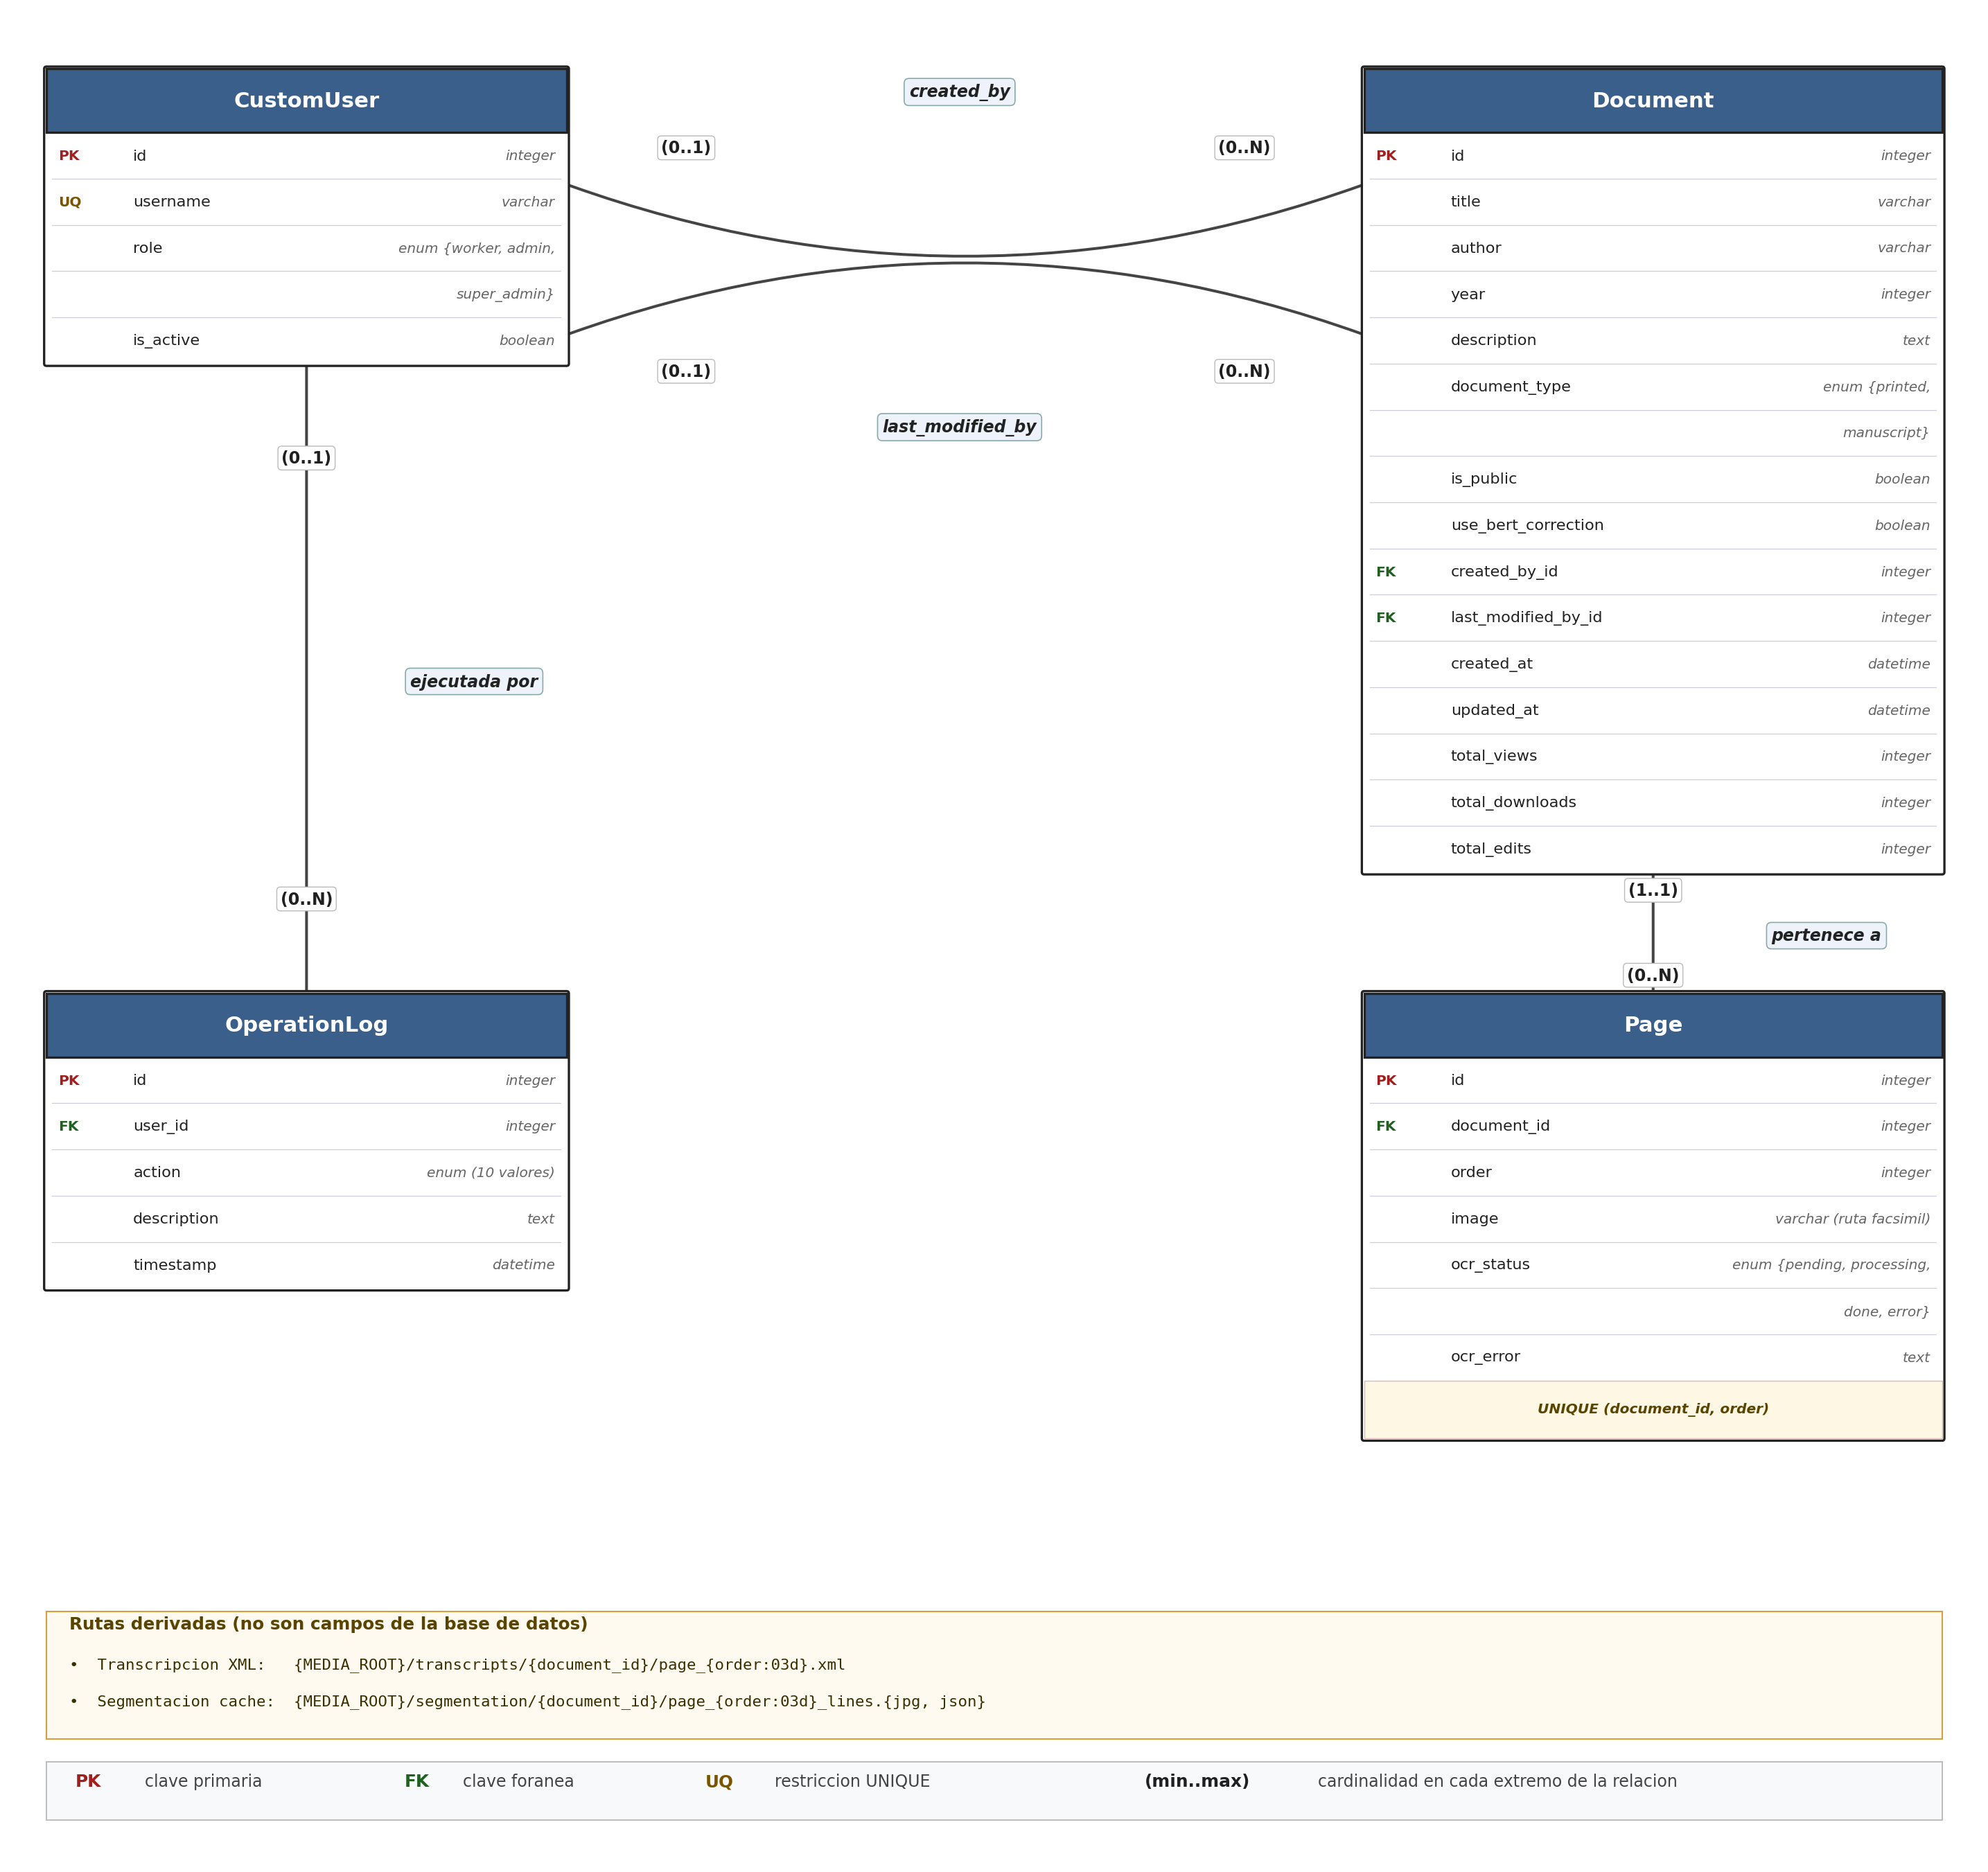
\includegraphics[width=\textwidth]{Graphics/mer_diagram.png}
	\caption{Diagrama Modelo Entidad-Relación del esquema relacional de la aplicación web. Las claves primarias se marcan con \textcolor{red!60!black}{\textbf{PK}}, las claves foráneas con \textcolor{green!40!black}{\textbf{FK}} y las restricciones de unicidad con \textcolor{orange!60!black}{\textbf{UQ}}. Cada línea entre dos entidades representa una relación, con la cardinalidad mínima y máxima entre paréntesis en cada extremo. La nota al pie del diagrama documenta las dos rutas que se derivan del identificador del documento y del orden de la página, sin almacenarse como campos en la base de datos.}
	\label{fig:mer-diagrama}
\end{figure}

\subsection{Documentos y páginas}
\label{subsec:documentos-paginas}

La entidad documento representa una obra digitalizada del archivo del centro Juan Marinello: un libro, una revista, un expediente, una carta u otro tipo de archivo. Cada documento agrupa una o más páginas. Los atributos principales del documento son el título, el año de publicación, el autor, una descripción libre, el tipo del documento, un indicador de visibilidad pública, y referencias al usuario que lo creó y al último que lo modificó. El tipo del documento toma uno de dos valores: \textit{impreso} o \textit{manuscrito}. El presente trabajo cubre únicamente el caso impreso; el caso manuscrito queda fuera del alcance y el capítulo no lo desarrolla.

El indicador de visibilidad pública gobierna el acceso de los usuarios no autenticados. Un documento público es visible para cualquier visitante del sitio sin necesidad de registro, mientras que un documento privado requiere autenticación con un rol que disponga del permiso de lectura. El indicador permite al centro mantener parte del archivo en consulta abierta y reservar el resto a usuarios institucionales.

La entidad página representa un facsímil individual dentro de un documento. Cada página almacena su número de orden dentro del documento, la imagen facsimilar, y el estado del procesamiento OCR. El estado toma uno de cuatro valores: \textit{pendiente}, \textit{en proceso}, \textit{listo} o \textit{error}. La transición entre estados la gestiona el componente que coordina las tareas en \textit{background}, que la sección~\ref{sec:flujo-digitalizacion} describe.

El texto que el OCR produce, junto con las regiones que el usuario pueda definir sobre la página, no descansa en la base de datos relacional sino en un fichero XML por página. La sección~\ref{sec:formato-xml} desarrolla la decisión y el formato del fichero. El acceso al texto desde el código opera mediante los métodos \texttt{get\_text} y \texttt{set\_text} que la página expone, los cuales delegan en una capa específica que encapsula toda la entrada y salida de ficheros XML. El resto del proyecto interactúa siempre a través de la página, sin tocar el sistema de ficheros directamente.

Una segunda categoría de ficheros que el sistema vincula a cada página son las visualizaciones de la segmentación de líneas, que el editor de revisión emplea para superponer las cajas de líneas sobre el facsímil. El sistema calcula la visualización la primera vez que el editor la solicita, junto con un fichero JSON que contiene las coordenadas exactas de las cajas, y guarda ambos en el subdirectorio \texttt{segmentation/} de la ruta del documento. La estrategia evita recalcular la segmentación en cada apertura del editor.

\subsection{Registro de operaciones y métricas de uso}
\label{subsec:auditoria}

El sistema mantiene un registro de auditoría con todas las operaciones que modifican el estado del archivo: inserción, edición o eliminación de documentos, inserción o eliminación de usuarios, cambios de privilegios, y eventos de inicio y cierre de sesión. Cada entrada del registro guarda el usuario que ejecutó la acción, el tipo de acción según un catálogo cerrado, una descripción textual del cambio, y la marca de tiempo. El registro permite reconstruir la historia de cualquier documento ante una incidencia y atribuir responsabilidades cuando varios usuarios colaboran sobre el mismo material.

Las métricas de uso complementan al registro de auditoría con tres contadores incrementales por documento: el número total de visualizaciones, el número total de descargas y el número total de ediciones. Los tres contadores los actualiza el código en las vistas correspondientes mediante operaciones atómicas que evitan condiciones de carrera entre peticiones simultáneas. Las métricas alimentan los paneles de la aplicación \textit{stats} y orientan al equipo del centro sobre los materiales con mayor número de consultas.

El sistema garantiza la coherencia entre la base de datos relacional y los ficheros del sistema durante las operaciones de borrado mediante \textit{signals} de Django que conectan al evento \textit{post-delete}. Cuando la base de datos elimina una página, un manejador borra el fichero del facsímil, el fichero XML de transcripción y los ficheros de la visualización de segmentación que la caché guarda. Cuando la base elimina un documento, el borrado en cascada del modelo relacional propaga la eliminación a todas sus páginas, y un segundo manejador limpia los directorios del documento en los tres subdirectorios \texttt{facsimiles/}, \texttt{transcripts/} y \texttt{segmentation/} por si hubiera quedado algún fichero huérfano de procesos anteriores. El mecanismo evita la acumulación de ficheros sin referencia en disco a medida que el archivo crece o las operaciones de reorganización avanzan.

% -----------------------------------------------------------------------------
\section{Roles de usuario y control de acceso}
\label{sec:roles-acceso}

El sistema distingue tres roles para los usuarios autenticados: trabajador, administrador y administrador principal. Cada rol amplía las capacidades del anterior. La tabla~\ref{tab:roles} resume las capacidades concretas de cada rol.

\begin{table}[!htbp]
	\centering
	\caption{Capacidades que el sistema concede a cada rol.}
	\label{tab:roles}
	\begin{tabular}{lp{10cm}}
		\toprule
		\textbf{Rol} & \textbf{Capacidades} \\
		\midrule
		Trabajador & Sube documentos nuevos, ejecuta OCR sobre las páginas, edita y corrige las transcripciones que el modelo produce, elimina documentos del archivo y descarga el contenido del archivo. \\
		\addlinespace
		Administrador & Las del trabajador y, adicionalmente, gestiona los usuarios con rol de trabajador, accede al registro de operaciones y a las métricas de uso. \\
		\addlinespace
		Administrador principal & Las del administrador y, adicionalmente, crea o elimina otros administradores. La instalación inicial del sistema crea un administrador principal mediante un comando específico de la línea de órdenes de Django. \\
		\bottomrule
	\end{tabular}
\end{table}

El sistema aplica el control de acceso mediante decoradores que envuelven las vistas. Cada vista declara el rol mínimo que requiere para ejecutarse. Cuando un usuario sin el rol suficiente intenta acceder, el decorador devuelve una respuesta de denegación con el código de estado apropiado, sin que el código de la vista llegue a ejecutarse. La estrategia centraliza la lógica de autorización y evita la dispersión de comprobaciones a lo largo del proyecto.

Los visitantes que no se autentican pueden consultar y descargar los documentos públicos, así como buscar dentro de su contenido. La distinción permite al centro publicar parte del archivo sin obligar a los lectores ocasionales a registrarse, mientras se reserva el material no público a los usuarios con rol institucional.

% -----------------------------------------------------------------------------
\section{Flujo de digitalización}
\label{sec:flujo-digitalizacion}

El flujo completo que recorre un documento desde su entrada al sistema hasta su consulta final comprende cinco fases: subida, procesamiento OCR asíncrono, revisión manual, almacenamiento y consulta. La figura~\ref{fig:flujo-digitalizacion} resume las cinco fases en secuencia; los párrafos siguientes las desarrollan en detalle.

\begin{figure}[!htbp]
	\centering
	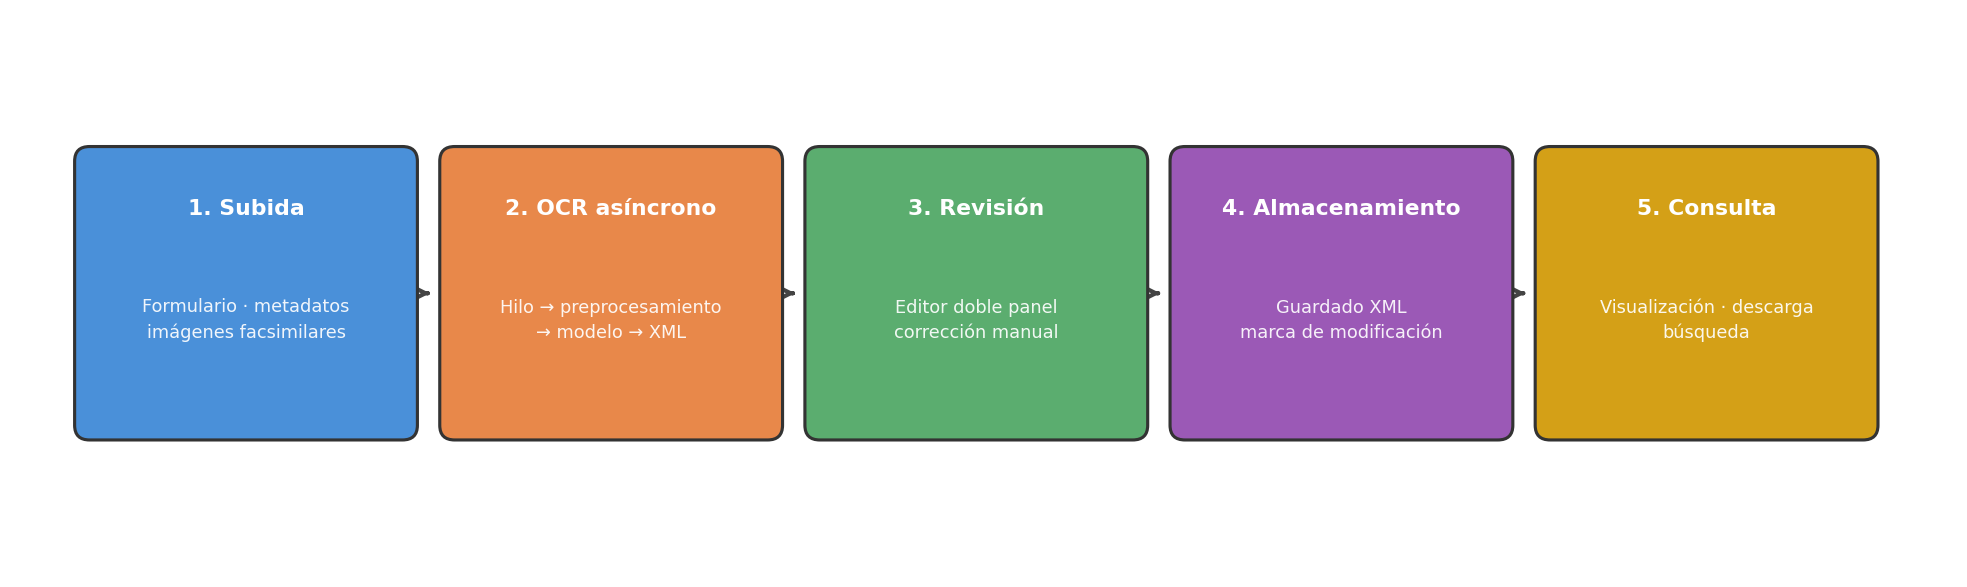
\includegraphics[width=\textwidth]{Graphics/flujo_digitalizacion.png}
	\caption{Las cinco fases del flujo de digitalización: subida, procesamiento OCR asíncrono, revisión manual, almacenamiento y consulta.}
	\label{fig:flujo-digitalizacion}
\end{figure}

La fase de subida la inicia el usuario al crear un documento nuevo mediante el formulario de inserción. El usuario aporta los metadatos del documento y selecciona las imágenes facsimilares correspondientes a las páginas. El \textit{framework} valida los formularios mediante el sistema declarativo de validación de Django, persiste los metadatos del documento y de las páginas en la base de datos, y guarda cada imagen en el sistema de ficheros bajo una ruta determinista que organiza los facsímiles por documento. Las páginas que la subida crea quedan inicialmente en estado pendiente, sin transcripción.

La fase de procesamiento OCR la inicia el sistema inmediatamente después de la subida, sin intervención del usuario. La invocación del OCR sobre todas las páginas de un documento de cien páginas, ejecutada de forma sincrónica dentro de la petición HTTP~\cite{ietf2022http}, tardaría varios minutos y desbordaría los tiempos de respuesta habituales. La aplicación adopta en su lugar un esquema asíncrono basado en hilos. Cuando el usuario completa la subida, la vista correspondiente arranca un hilo propio del documento, devuelve la respuesta HTTP inmediatamente y libera al usuario para que continúe trabajando o consulte el progreso. El hilo recorre las páginas pendientes por orden, marca cada una como en proceso, ejecuta el OCR, almacena la transcripción y deja la página en estado listo, o en estado error si el procesamiento falla. La interfaz consulta periódicamente el estado del documento y desbloquea cada página a medida que el hilo la completa.

El esquema basado en hilos presenta una limitación frente a una cola de tareas externa con persistencia propia y \textit{workers} independientes del proceso del servidor web: si el proceso de Django muere a mitad del procesamiento, las páginas que estaban en proceso quedan huérfanas con su estado intermedio. El sistema mitiga la limitación mediante una rutina de recuperación que arranca con el servidor: la rutina detecta las páginas que llevan más de un umbral de tiempo en estado de procesamiento, las marca de vuelta como pendientes, y desencadena un nuevo intento sobre los documentos afectados. El esquema sin cola externa resulta adecuado para volúmenes moderados de subidas simultáneas como los que el contexto del centro Juan Marinello espera; un crecimiento sustancial de la demanda justificaría la migración a una infraestructura con cola persistente y \textit{workers} específicos del procesamiento OCR.

La aplicación admite además la cancelación del procesamiento cuando el usuario decide abandonar un documento durante la subida. La vista de abandono inserta el identificador del documento en un conjunto de cancelaciones pendientes que el hilo del OCR consulta entre página y página: cuando el identificador aparece en el conjunto, el hilo termina de procesar la página actual y sale del bucle sin tocar las páginas pendientes. El procesamiento de la página en curso no admite interrupción a la fuerza porque el modelo de PyTorch no soporta interrupción limpia a mitad de inferencia. Una vez cancelado, el documento admite eliminación mediante la vista correspondiente, que el sistema concede a cualquier usuario con rol de trabajador o superior.

Además del procesamiento automático al subir el documento, la aplicación ofrece dos botones en el editor que permiten al usuario lanzar el OCR sobre alcances más estrechos. El primero, identificado como \emph{Re-ejecutar OCR}, reprocesa la página que el usuario tiene abierta; el sistema la marca de vuelta como pendiente, ejecuta el \textit{pipeline} completo y actualiza la transcripción cuando termina. El segundo, identificado como \emph{OCR de regiones}, restringe el reconocimiento a las cajas que el usuario haya dibujado sobre el facsímil y sustituye la transcripción de la página con el texto que produce cada región en el orden que el usuario asignó. Ambos botones comparten el mismo motor OCR y la misma capa de persistencia que el procesamiento inicial. La figura~\ref{fig:editor-botones} ilustra su posición en la interfaz del editor.

\begin{figure}[!htbp]
	\centering
	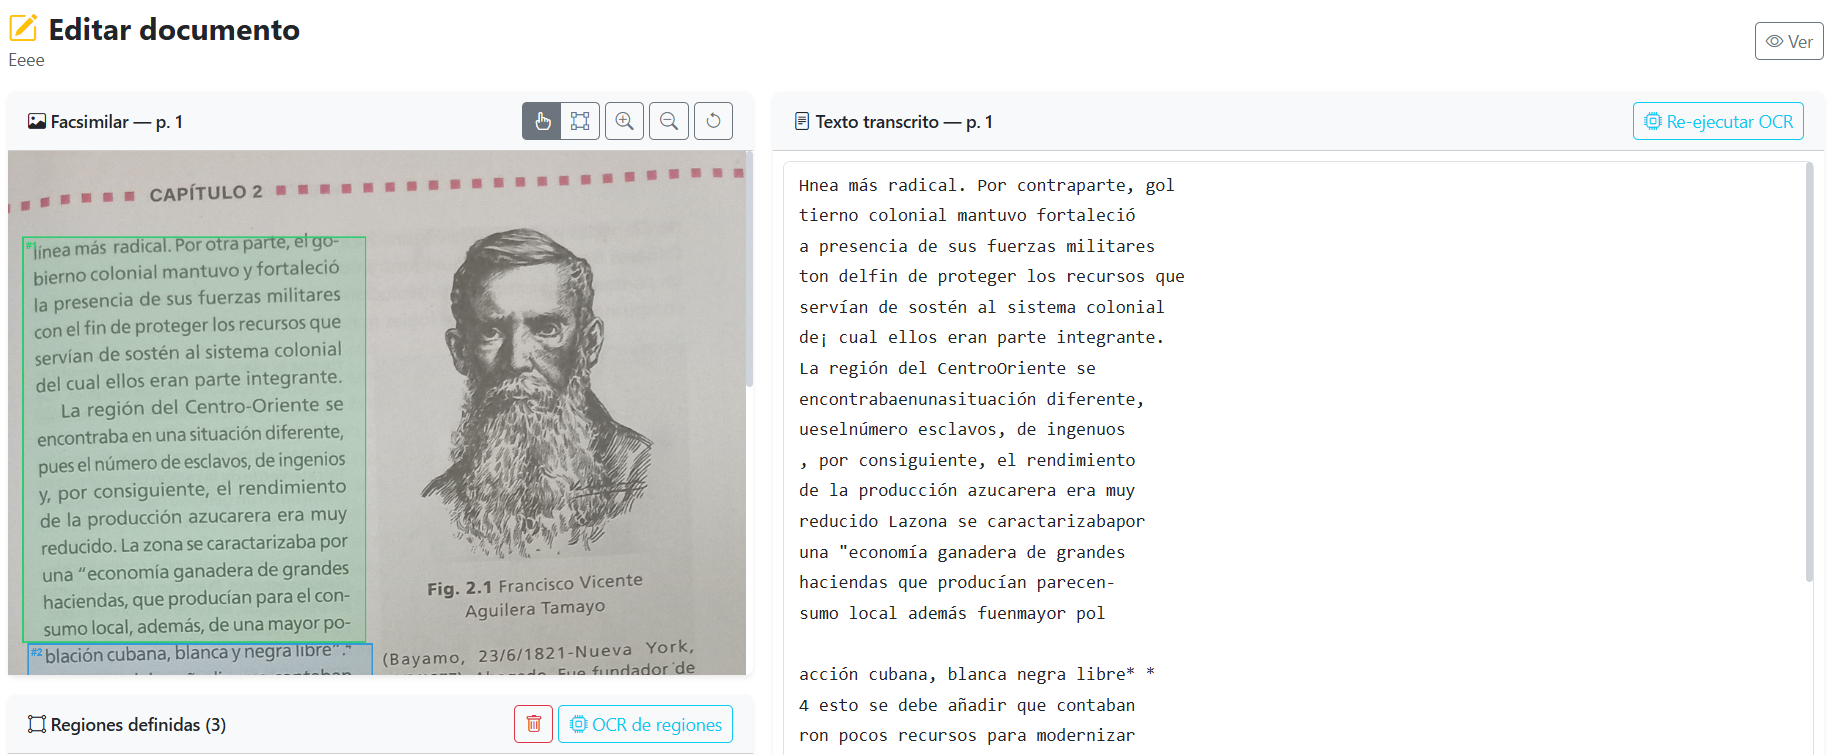
\includegraphics[width=0.92\textwidth]{Graphics/editor_botones.png}
	\caption{Botones de reconocimiento del editor: \emph{Re-ejecutar OCR} (panel derecho, esquina superior) para reprocesar la página completa, y \emph{OCR de regiones} (panel izquierdo, sección de regiones) para restringir el reconocimiento a las cajas que el usuario haya definido.}
	\label{fig:editor-botones}
\end{figure}

La fase de revisión manual la inicia el usuario al abrir la página de edición de cualquier página que ya esté en estado listo. La interfaz presenta al usuario el facsímil junto a la transcripción que el modelo produjo en un diseño de doble panel, y permite corregir los errores de reconocimiento. La figura~\ref{fig:editor-facsimil} muestra el aspecto del editor una vez que el OCR ha completado la página. Las características detalladas del editor se desarrollan en la sección~\ref{sec:editor}.

\begin{figure}[!htbp]
	\centering
	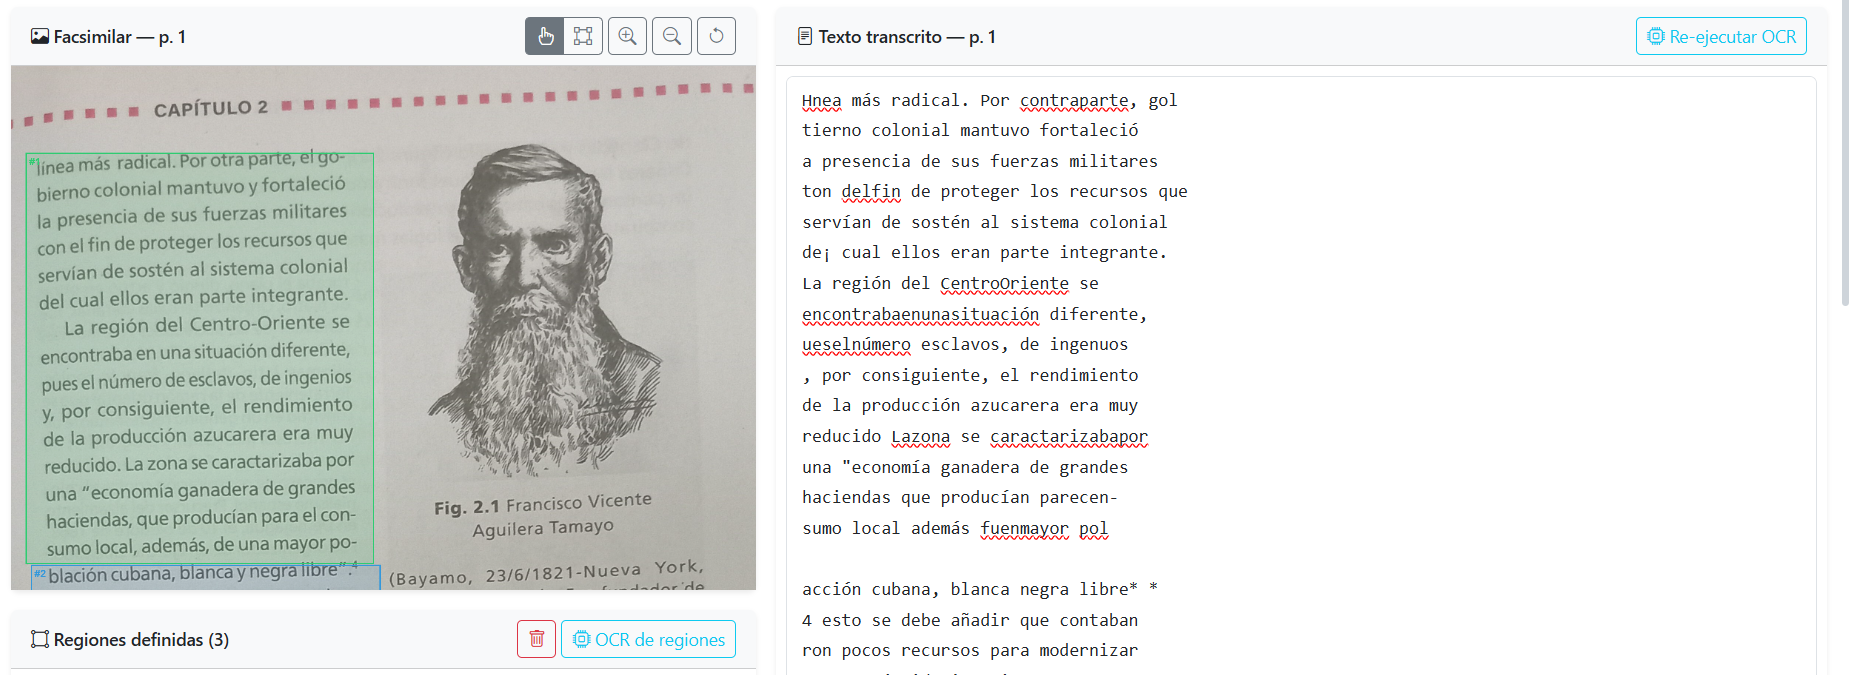
\includegraphics[width=0.9\textwidth]{Graphics/editor_facsimil_transcripcion.png}
	\caption{Editor de revisión con diseño de doble panel: el facsímil de la página en el panel izquierdo y la transcripción que el modelo produjo en el panel derecho, disponible para edición.}
	\label{fig:editor-facsimil}
\end{figure}

La fase de almacenamiento opera al guardar las correcciones del usuario. El sistema persiste las correcciones del usuario en el fichero XML correspondiente a la página, mediante la capa de transcripciones que la subsección~\ref{subsec:documentos-paginas} mencionó. La capa preserva los metadatos del documento y la marca de creación original del fichero, y actualiza la marca de última modificación.

La fase de consulta agrupa las acciones de lectura sobre el archivo ya digitalizado: visualización del documento por sus páginas, descarga del facsímil o de la transcripción, y búsqueda por título o contenido. Cada visualización incrementa el contador de visualizaciones del documento, cada descarga incrementa el contador de descargas, y cada edición incrementa el contador de ediciones, según describió la subsección~\ref{subsec:auditoria}.

% -----------------------------------------------------------------------------
\section{Integración del modelo de reconocimiento}
\label{sec:integracion-ocr}

La integración del modelo de reconocimiento que el capítulo~\ref{chap:modelo} desarrolla con la aplicación web requiere tres puntos de articulación: la carga del modelo en memoria, la invocación del \textit{pipeline} de preprocesamiento, y la composición del texto reconocido para su almacenamiento.

La carga del modelo en memoria opera al arranque del proceso Django, no en respuesta a la primera petición. La estrategia evita que el primer usuario que invoca el OCR sufra una latencia inicial de varios segundos por la lectura de los pesos del modelo. Cuando el servidor Django arranca, un hilo en \textit{background} ejecuta una rutina de precarga que invoca los cinco modelos del sistema en un orden fijo: el modelo de lenguaje de \textit{n}-gramas a nivel de carácter, que el equipo entrenó previamente sobre \textit{corpus} de español de uso general y que la herramienta KenLM~\cite{heafield2011kenlm} carga; el corrector ortográfico SymSpell~\cite{garbe2012symspell}; el modelo CRNN+CTC~\cite{shi2016crnn,graves2006ctc} para impresos que el capítulo~\ref{chap:modelo} desarrolla; el modelo HTR para manuscritos --que queda fuera del alcance de esta tesis-- y el \textit{reranker} neuronal sobre BETO~\cite{canete2020beto}. La precarga ocurre en \textit{background} para no bloquear el arranque del servidor, y los cinco modelos quedan como singletons disponibles para las peticiones que llegan después. Cada singleton incorpora un mecanismo de bloqueo con doble verificación que protege contra cargas concurrentes en el caso de que una petición OCR llegue antes de que la precarga termine: la petición simplemente espera al bloqueo sin iniciar una segunda carga del mismo modelo. La inicialización lee los pesos que el entrenamiento del capítulo~\ref{chap:modelo} produjo y los carga en el dispositivo de cómputo que la instalación configura, que es la CPU por defecto pero puede ser una GPU si la instalación dispone de ella.

La invocación del \textit{pipeline} de preprocesamiento sobre cada página sigue las cinco etapas que el capítulo~\ref{chap:preprocesamiento} describió: análisis y configuración automática, binarización, corrección de inclinación a tres niveles, detección y segmentación de bloques y líneas, y normalización de cada línea para inferencia. La salida del \textit{pipeline} es una lista ordenada de líneas con altura uniforme de sesenta y cuatro píxeles y anchos variables, en el formato exacto que el modelo del capítulo~\ref{chap:modelo} espera como entrada.

La inferencia del modelo opera sobre las líneas en lotes para amortizar el coste fijo de cada llamada al dispositivo de cómputo. Cada lote agrupa líneas de anchos similares para reducir el desperdicio de relleno, según una estrategia análoga a la del muestreador por agrupamiento que la subsección~
ef{subsec:bucketing} describió. La decodificación adopta la búsqueda en haz con el modelo de lenguaje de cinco gramas que la subsección~\ref{subsec:lm-posterior} describe, configuración que mejora el rendimiento sobre documentos reales gracias a la mayor incertidumbre acústica del modelo visual ante degradaciones de escaneado y a la regularidad morfológica del español.

La composición del texto para su almacenamiento concatena las transcripciones de las líneas individuales con saltos de línea, preservando el orden vertical que el \textit{pipeline} estableció durante la segmentación. La concatenación pasa por la capa de transcripciones, que escribe el fichero XML correspondiente con el texto, los metadatos del documento y la marca de tiempo de creación.

La aplicación admite además una variante del procesamiento que opera sobre regiones definidas por el usuario en lugar de sobre la página completa. La variante resulta útil cuando el usuario quiere transcribir solamente una porción del facsímil, como un párrafo de interés dentro de un documento extenso o un fragmento legible dentro de una página parcialmente dañada. El usuario marca las regiones en el editor mediante el ratón, el sistema las guarda en el XML como cajas con coordenadas en píxeles del facsímil original, y el motor de OCR recorta cada caja antes de procesarla con el mismo \textit{pipeline} de preprocesamiento. La salida produce un texto que respeta el orden que el usuario asignó a las regiones.

El procesamiento de cada página por el motor OCR aplica un postprocesado al texto que la decodificación con búsqueda en haz y modelo de lenguaje produce, antes de almacenarlo. El postprocesado consta de un paso obligatorio y un paso opcional. El paso obligatorio es la corrección ortográfica mediante SymSpell~\cite{garbe2012symspell}, un corrector basado en distancia de edición y diccionario de frecuencias del español. SymSpell propone candidatos para cada palabra que no aparece en el diccionario y los ordena por una combinación de proximidad ortográfica y frecuencia en el idioma. El paso opcional es el \textit{reranking} neural: las palabras con varios candidatos plausibles se desambiguan mediante un modelo de lenguaje contextual basado en BETO que evalúa cada candidato en el contexto de la oración completa. La opción mejora la calidad en casos ambiguos a costa de una latencia adicional por página.

% -----------------------------------------------------------------------------
\section{Editor de revisión de transcripciones}
\label{sec:editor}

El reconocimiento automático rara vez produce una transcripción perfecta. Los errores residuales típicos incluyen confusiones entre signos de puntuación visualmente similares y omisión de tildes en cuerpos tipográficos pequeños, según se identificó en la sección~\ref{sec:fine-tuning} del capítulo anterior, junto con errores en regiones con tinta desvanecida o sangrado severo cuando la calidad del facsímil cae fuera del rango que el preprocesamiento puede compensar. La aplicación incorpora un editor de revisión que permite al usuario corregir los errores residuales con la imagen original visible como referencia.

El editor adopta un diseño de doble panel. El panel izquierdo muestra el facsímil de la página a tamaño completo, con la posibilidad de hacer zoom y desplazamiento mediante el ratón y el teclado. El panel derecho contiene un área de texto editable con la transcripción que el modelo produjo. El usuario lee la transcripción mientras consulta el facsímil para verificar las dudas, modifica los caracteres incorrectos en el área de texto, y guarda los cambios cuando termina la revisión de la página. La interfaz no impone separación rígida entre líneas: el área de texto presenta la transcripción como un cuerpo continuo que el usuario edita como cualquier texto plano. La figura~\ref{fig:editor-completo} muestra el editor con ambos paneles activos.

\begin{figure}[!htbp]
	\centering
	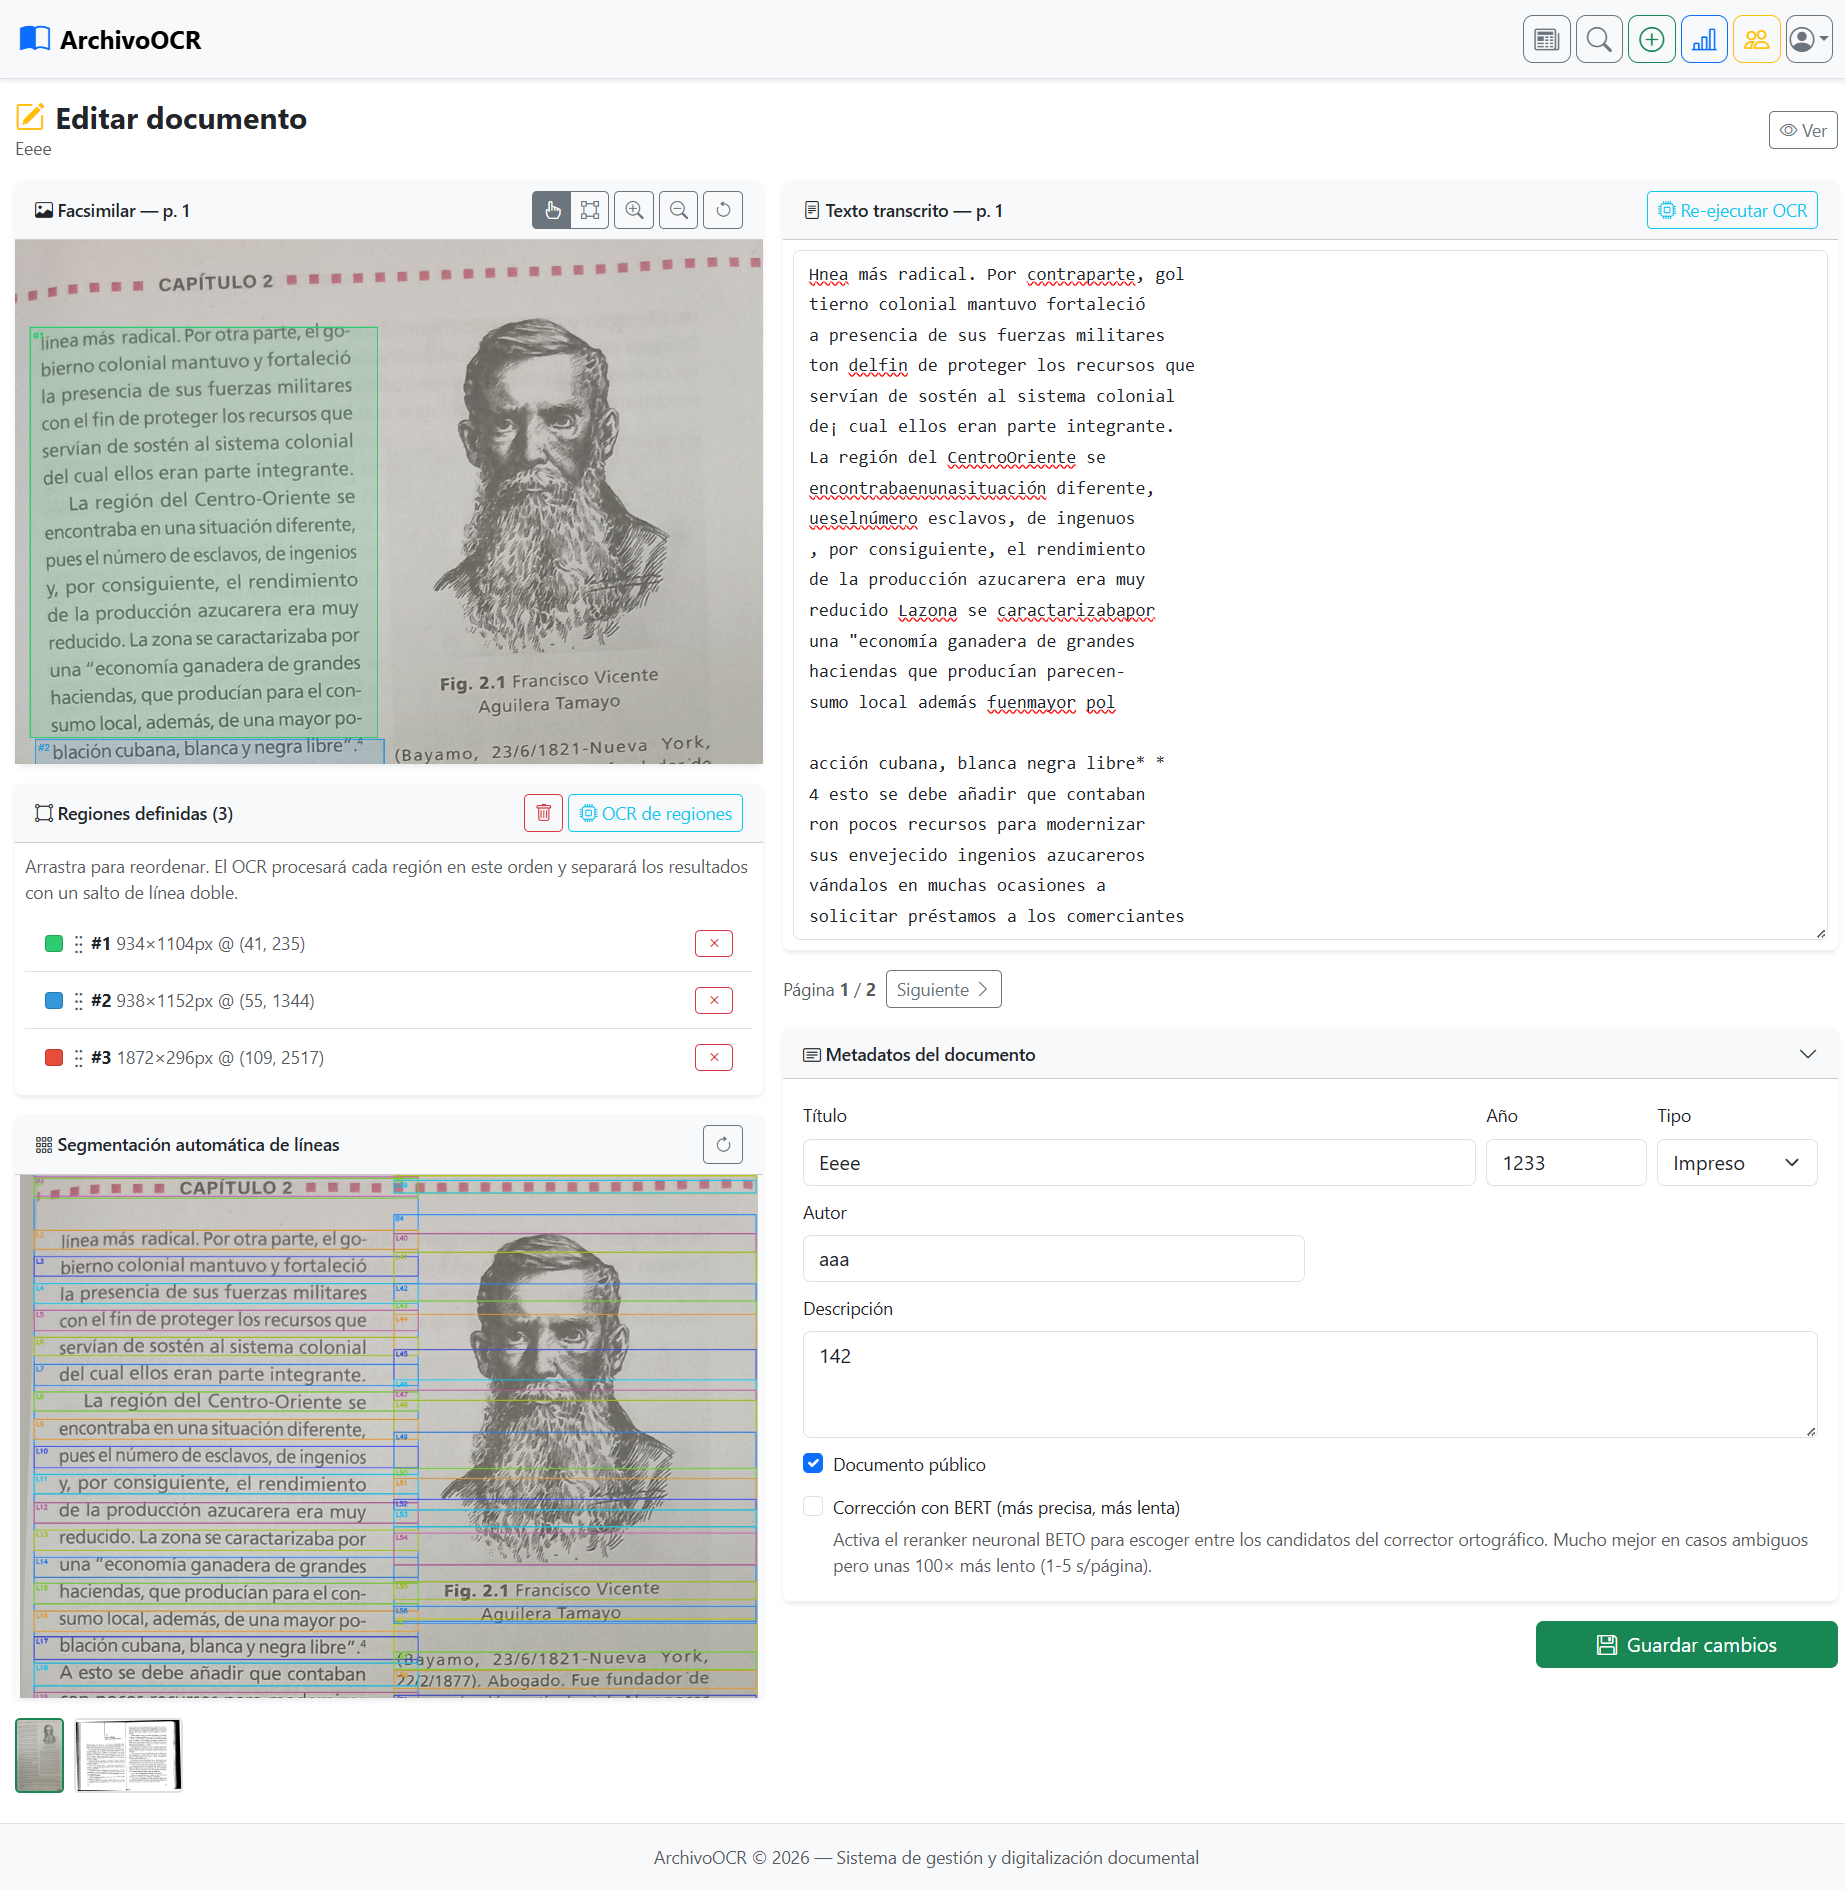
\includegraphics[width=0.78\textwidth]{Graphics/editor_completo.png}
	\caption{Vista completa del editor de revisión con el facsímil de la página arriba y la visualización de segmentación de líneas abajo en el panel izquierdo, y el texto que el modelo produjo en el panel derecho, junto al aviso de guardado.}
	\label{fig:editor-completo}
\end{figure}

Una segunda funcionalidad del editor permite visualizar la segmentación de líneas que el \textit{pipeline} de preprocesamiento produjo sobre la página. La visualización superpone, sobre el facsímil del panel izquierdo, las cajas que delimitan cada línea según la detección del capítulo~\ref{chap:preprocesamiento}. La superposición resulta útil para diagnosticar problemas de segmentación: una línea que el sistema no detectó, dos líneas que se unieron en una sola, o una caja desplazada respecto al texto. El usuario puede entonces volver al material físico, escanear la página en mejores condiciones, o aceptar el resultado tras valorar la magnitud del error. La figura~\ref{fig:editor-segmentacion} muestra la visualización de segmentación superpuesta sobre el facsímil.

\begin{figure}[!htbp]
	\centering
	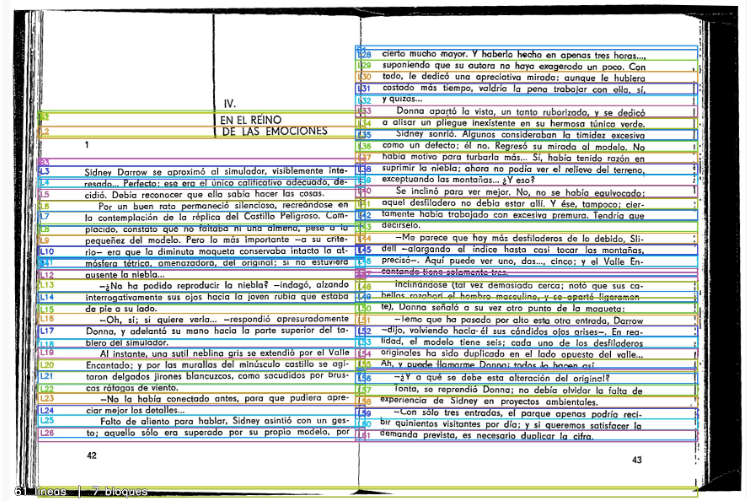
\includegraphics[width=0.6\textwidth]{Graphics/editor_segmentacion.png}
	\caption{Panel izquierdo del editor con la visualización de segmentación activa. Cada caja de color delimita una línea que el \textit{pipeline} del capítulo~\ref{chap:preprocesamiento} detectó; las etiquetas L1, L2,~\ldots{} identifican el orden de lectura.}
	\label{fig:editor-segmentacion}
\end{figure}

El editor incorpora una protección contra escrituras concurrentes cuando el OCR aún está en curso sobre el documento. Mientras alguna página del documento permanece en estado pendiente, en proceso o de error, el editor permite al usuario navegar entre páginas pero rechaza cualquier intento de guardar cambios sobre el texto. La protección evita que el hilo del OCR, al terminar de procesar una página, sobrescriba con su transcripción el texto que el usuario hubiera comenzado a editar manualmente en la misma página. Una vez que todas las páginas alcanzan el estado de listas, el editor desbloquea el guardado y el usuario puede corregir libremente las transcripciones.

La definición de regiones por el usuario, que el final de la sección anterior mencionó, también opera en el editor. El usuario arrastra el ratón sobre el facsímil para dibujar cajas, asigna el orden con que quiere que el sistema las procese, y desencadena el reconocimiento, que el sistema restringe a las regiones que el usuario dibujó. El resultado sustituye, en el área de texto, a la transcripción anterior de la página.

Más allá de la edición de la transcripción, el editor ofrece tres operaciones complementarias sobre el documento. La primera es el abandono de la edición, que descarta los cambios que el usuario todavía no ha guardado. La segunda es la eliminación del documento, disponible para cualquier usuario con rol de trabajador o superior, según se detalló en la sección~\ref{sec:roles-acceso}. La tercera es la descarga del documento, que produce un documento PDF~\cite{iso2020pdf} o EPUB~\cite{w3c2023epub} con la transcripción completa del archivo, con la opción adicional de incluir los facsímiles originales junto al texto.

% -----------------------------------------------------------------------------
\section{Formato XML y exportación a estándares}
\label{sec:formato-xml}

La transcripción de cada página se almacena en un fichero XML independiente, según se introdujo en la subsección~\ref{subsec:documentos-paginas}. La presente sección desarrolla la estructura del fichero y las decisiones de diseño que la sustentan.

\subsection{Estructura del fichero}
\label{subsec:estructura-xml}

El fichero XML de una página contiene cinco bloques principales: un identificador del documento al que pertenece, los metadatos básicos como título, autor, año y tipo, una referencia al facsímil de la página, las marcas de tiempo de creación y última modificación, y el cuerpo de la transcripción organizado en líneas. Un bloque opcional adicional almacena las regiones que el usuario haya definido sobre la página. El esquema completo se ilustra en el siguiente fragmento:

\begin{lstlisting}[language=XML,caption={Estructura del fichero XML de transcripción por página.},label={lst:xml}]
	<?xml version="1.0" encoding="UTF-8"?>
	<Transcript version="1">
	<Document id="42">
	<Title>Don Quijote de la Mancha</Title>
	<Author>Miguel de Cervantes</Author>
	<Year>1605</Year>
	<Type>printed</Type>
	</Document>
	<Page order="3" facsimile="page_003.jpg"/>
	<Timestamps>
	<Created>2026-05-09T14:30:00+02:00</Created>
	<Modified>2026-05-09T14:35:12+02:00</Modified>
	</Timestamps>
	<Regions>
	<Region id="r1" order="1" x="120" y="80" width="900" height="220"/>
	</Regions>
	<Body>
	<Line>En un lugar de la Mancha, de cuyo nombre no quiero acordarme,</Line>
	<Line>no ha mucho tiempo que vivia un hidalgo de los de lanza en astillero,</Line>
	<Line/>
	<Line>adarga antigua, rocin flaco y galgo corredor.</Line>
	</Body>
	</Transcript>
\end{lstlisting}

Cada \texttt{Line} representa un salto lógico de línea. Las líneas vacías que el OCR detecta como separación entre párrafos permanecen como elementos \texttt{Line} sin contenido. La representación en texto plano resulta de concatenar el contenido de los elementos \texttt{Line} con saltos de línea.

\subsection{Decisiones de diseño}
\label{subsec:decisiones-xml}

El esquema responde a tres objetivos. El primer objetivo es la legibilidad humana directa. Un revisor puede abrir cualquier fichero con un editor de texto y entender el contenido sin herramientas auxiliares, lo que reduce la barrera para auditar o reparar manualmente las transcripciones cuando aparece una incidencia. El segundo objetivo es la independencia de bibliotecas externas. La serialización emplea \texttt{ElementTree}, la biblioteca XML que viene con la distribución estándar de Python, sin requerir paquetes adicionales como \texttt{lxml}. El tercer objetivo es la convertibilidad a estándares mayores en caso de que el archivo crezca y requiera interoperabilidad institucional.

La decisión de mantener las transcripciones en ficheros XML y no en filas de la base de datos relacional merece justificación. Los argumentos a favor del XML son tres. Primero, el contenido de una transcripción se consulta casi siempre por su clave de página, no por sus contenidos internos; la base de datos relacional ofrece poca ventaja sobre el sistema de ficheros cuando el patrón de acceso es siempre por clave única. Segundo, el XML resulta inmediatamente exportable, lo que facilita las copias de seguridad y la migración a otro almacenamiento. Tercero, la versión textual de la transcripción puede crecer sin afectar el tamaño de las tablas relacionales, lo que mantiene la base de datos compacta y eficiente para las consultas que sí requieren índices.

Una ventaja adicional del esquema propio es que el conjunto de información que captura constituye un subconjunto de los estándares ALTO~\cite{loc-alto}, PAGE-XML~\cite{pletschacher2010page} y TEI~\cite{tei-consortium}, que los archivos digitales emplean ampliamente. La elección preserva la posibilidad de que el archivo del centro Juan Marinello migre a cualquiera de los tres estándares cuando el sistema se integre en un repositorio institucional con requisitos de interoperabilidad, sin pérdida de información respecto al estado actual.

% -----------------------------------------------------------------------------
% Cierre del capítulo
% -----------------------------------------------------------------------------

La aplicación web que el capítulo describe completa el sistema con la capa de interacción con el usuario. El conjunto del trabajo, desde la generación del \textit{corpus} sintético del capítulo~\ref{chap:corpus} hasta la integración en la aplicación que el capítulo~\ref{chap:web} desarrolla, configura una herramienta operativa para la digitalización del archivo del centro Juan Marinello. Las contribuciones del trabajo, las limitaciones que se identificaron y las líneas de trabajo que quedan abiertas se sintetizan en las conclusiones que cierran el documento.
